\documentclass[./main.tex]{subfiles}
\begin{document}
\chapter{Analytical treatment of equations of motion in \textit{Gorilla}}
\section{Analytical solution of equations of motion}
\label{sec:analytical_solution}
\noindent
In this section, an analytic solution to the linear equations of motion within a tetrahedron will be derived, following the formulation of guiding center equations by \textit{Solov'ev} and \textit{Morozov} \cite{Revies_Plasma_Vol2} and the local linearization by M. Eder \textit{et al} \cite{Eder_EPS}. \\
By denoting the extended set of variables with $z^i$, where $z^i=x^i$ for $i=1,2,3$ and $z^4=v_\parallel$, the linearized equation set assumes a standard form
\be{standeqset}
\frac{\rd z^i(\tau)}{\rd \tau} = a^i_l(\tau) z^l(\tau) + b^i,
\ee
where for $i,l=1,2,3$ the matrix elements are


\bea{amatdef}
a^i_l &=& \varepsilon^{ijk}\left(
2\difp{U}{x^l}\difp{}{x^j}\frac{B_k}{\omega_c}+\difp{U}{x^j}\difp{}{x^l}\frac{B_k}{\omega_c}
\right) 
\qquad\mbox{for}\qquad 1\le i,l \le 3,
\nonumber \\
a^i_4 &=& \varepsilon^{ijk} \difp{A_k}{x^j}
\qquad\mbox{for}\qquad 1\le i \le 3,
\nonumber \\
a^4_l &=& 0 
\qquad\mbox{for}\qquad 1\le l \le 3,
\nonumber \\
a^4_4 &=& \varepsilon^{ijk}\difp{U}{x^i}
\difp{}{x^j}\frac{B_k}{\omega_c},
\eea


and the components of vector $b^i$ are
\bea{bvecdef}
b^i &=& \varepsilon^{ijk}\left(
2U_0\difp{}{x^j}\frac{B_k}{\omega_c}+\left(\frac{B_k}{\omega_c}\right)_0\difp{U}{x^j}
\right)
\qquad\mbox{for}\qquad 1\le i \le 3,
\nonumber \\
b^4 &=& \varepsilon^{ijk}\difp{U}{x^i}
\difp{A_k}{x^j}.
\eea

Mind, that for all $i,l = 1,..,4$ the coefficients $a^i_l$ and $b^i$ remain constant within the scope of pushing through a tetrahedron. More precisely, since $U = v_\parallel^2 / 2$, only $U_0$ (the value of $U$ at the first vertex of the tetrahedron) and the gradient $\partial U/\partial x^i$ depend on initial conditions ($x^i$, $v_\parallel$ and $v_\perp$) of the particle entering a given tetrahedron, all other quantities (as well as some components of U) are independent of initial conditions and, thus, can be precomputed upon generation of the array \texttt{tetra\_physics} in module \texttt{tetra\_physics\_mod}.

\subsection{Reduction to a set of three linear ODEs}
\noindent

One is now interested in finding an analytic expression for $z^i(\tau)$.

Here, one can start by looking at the fourth component which is the parallel velocity as a function of time. One can quickly show that this equation is in fact decoupled from $x^i$, allowing for it to be solved independently, resulting to
\be{defvpar}
v_\parallel(\tau)=\left(v_\parallel(0)+\frac{b}{a}\right)\textrm{e}^{a\tau}-\frac{b}{a},
\ee
with $a$ and $b$ being
$$
a = \varepsilon^{ijk}\difp{U}{x^i}\difp{}{x^j}\frac{B_k}{\omega_c},
\qquad
b = \varepsilon^{ijk}\difp{U}{x^i}\difp{A_k}{x^j},
$$

which are both constant within the linearized fields. For compactness, this expression will be abbreviated for further calculation using $\eta = (v_\parallel(0)+\frac{b}{a})$ and $\theta = (\frac{b}{a})$, thus,
\be{defvpar2}
v_\parallel(\tau)=\eta\textrm{e}^{a\tau}-\theta.
\ee


The set of differential equations can now be formulated in a way that all time dependence is confined to a driving term. In order to achieve this, one starts with equation \ref{standeqset} and takes only the first three components into account, which yield for $i = 1,2,3$

\bea{derivation of 3d set of equations} 
\frac{\textrm{d} x^i(\tau)}{\textrm{d}\tau} &=& a^i_lx^l(\tau) + a^i_4z^4(\tau) + b^i \\ \nonumber
&=& \underbrace{\varepsilon^{ijk}\left(2 \frac{\partial U}{\partial x^l}\frac{\partial}{\partial x^j}\frac{B_k}{\omega_c} + \frac{\partial U}{\partial x^j}\frac{\partial}{\partial x^l}\frac{B_k}{\omega_c}	\right)}_{=a^i_l}x^l(\tau) + \underbrace{\varepsilon^{ijk} \left( \frac{\partial A_k}{\partial x^j} \right)}_{= a^i_4} \underbrace{z^4(\tau)}_{=v_\parallel(\tau)}  
 \\ \nonumber
&+& \underbrace{\varepsilon^{ijk} \left( 2U_0 \frac{\partial}{\partial x^j}\frac{B_k}{\omega_c}+\left( \frac{B_k}{\omega_c}\right)_0\frac{\partial U}{\partial x^j} \right)}_{=b^i} .
\nonumber
\eea

Furthermore, using $U(x^i)= U_0 + x^i\frac{\partial U}{\partial x^i}$  and $U = \frac{v_\parallel ^2}{2}$ simplifies this equation to
\be{3d explicit DE for x} \nonumber
\frac{\textrm{d} x^i(\tau)}{\textrm{d}\tau} = \underbrace{\varepsilon^{ijk}\difp{U}{x^j}\difp{}{x^l}\frac{B_k}{\omega_c}}_{=\tilde{a}^i_l}x^l(\tau)+ \underbrace{v_\parallel(\tau) \varepsilon^{ijk}\frac{\partial A_k}{\partial x^j} + v_\parallel^2(\tau)\varepsilon^{ijk}\frac{\partial}{\partial x^j}\frac{B_k}{\omega_c} + \varepsilon^{ijk} \left( \frac{B_k}{\omega_c}\right)_0 \frac{\partial U}{\partial x^j}}_{q^i(\tau)},
\ee

which can be compactly written as

\be{short 3d de for x} 
\frac{\textrm{d} x^i(\tau)}{\textrm{d}\tau} = \tilde{a}^i_l x^l(\tau) + q^i(\tau),
\ee

where
\be{gammadef} 
\tilde{a}^i_l=\varepsilon^{ijk}\difp{U}{x^j}\difp{}{x^l}\frac{B_k}{\omega_c}
\ee
is a constant matrix
and the driving term $q^i(\tau)$ is explicitly given by 
\be{defqi}
q^i(\tau)=
\varepsilon^{ijk}\left(
v_\parallel(\tau)  \difp{A_k}{x^j}  +v_\parallel^2(\tau)\difp{}{x^j}\frac{B_k}{\omega_c}
+\left(\frac{B_k}{\omega_c}\right)_0\difp{U}{x^j}
\right).
\ee
For compactness, this is abbreviated as
\bea{defqi2} \nonumber
q^i(\tau)&=&v_\parallel(\tau) \underbrace{\varepsilon^{ijk} \left( \difp{A_k}{x^j}\right)}_{\alpha^i}  
+v_\parallel^2(\tau)   \underbrace{ \varepsilon^{ijk}       \difp{}{x^j}\frac{B_k}{\omega_c}}_{\beta^i} 
+ \underbrace{\varepsilon^{ijk} \left( \frac{B_k}{\omega_c}\right)_0\difp{U}{x^j}}_{\gamma^i} \\ 
&=&v_\parallel(\tau){\alpha^i}+v_\parallel^2(\tau) {\beta^i}+{\gamma^i}.
\eea
The terms $\alpha^i$, $\beta^i$ and $\gamma^i$ are constant within a tetrahedral cell, where the electromagnetic fields are linear. Thus, all time dependence arises therefore from $v_\parallel(\tau)$.


\subsection{Homogeneous solution to equation of motion}
\noindent
The next step of calculating the analytical solution to the homogeneous part of equation \ref{short 3d de for x} is to start with the following Ansatz
\be{Ansatzeq} 
\vec{x} = e^{\lambda\tau}\vec{\psi}~.
\ee
Using this, equation \ref{standeqset} yields the eigenvalue equation
\be{Ansatzeq2} 
\lambda e^{\lambda \tau}\vec{\psi} = \hat{a} e^{\lambda\tau}\vec{\psi}~,
\ee
where $\hat{a}$ denotes matrix $a^i_l$, $\lambda$ the associated eigenvalues and $\psi$ the eigenvectors, respectively.
Therefore, the general solution to the homogeneous differential equation can be written as
\be{eq:homogeneousSolution1_0} 
\vec{x}_{(h)}(\tau) = C_1e^{\lambda_1\tau}\vec{\psi_1} + C_2e^{\lambda_2\tau}\vec{\psi_2} + C_3e^{\lambda_3\tau}\vec{\psi_3}.
\ee
Here, the $C_l$ denote a vector of arbitrary constants given by initial conditions of the problem. 
Equation \ref{eq:homogeneousSolution1_0} can be rewritten using index notation
\be{} 
x^i_{(h)}(\tau) = \psi^i_l C^l e^{\lambda^l \tau},
\ee
where $\psi^i_l$ is a matrix with eigenvectors $\vec{\psi}_l$ as columns, each corresponding to the respective eigenvalues $\lambda^l$.

\subsection{Particular solution: variation of constants}
\noindent
Next, the particular solution to the inhomogeneous ordinary differential equation set \ref{standeqset} will be derived. In order to do this, the method of variation of constants is applied. With this approach, the coefficients $\widetilde{C}_l$ are treated as functions of $\tau$
\be{homogeneousSolution2} 
\vec{x}_{(p)}(\tau) = \widetilde{C}_1(\tau)e^{\lambda_1\tau}\vec{c_1} + \widetilde{C}_2(\tau)e^{\lambda_2\tau}\vec{c_2} + \widetilde{C}_3(\tau)e^{\lambda_3\tau}\vec{c_3},
\ee
which again can be denoted in index notation
\be{}
x^i_{(p)}(\tau) = \psi^i_l \widetilde{C}^l(\tau) e^{\lambda^l \tau}. 
\ee
Calculating the derivative of this equation yields
\be*
\begin{split}
\frac{\mathrm{d}\vec{x}} {\mathrm{d}\tau} &= {\widetilde{C}_1}^\prime(\tau)e^{\lambda_1\tau}\vec{\psi_1}+ \widetilde{C}_1(\tau)\lambda_1e^{\lambda_1\tau}\vec{\psi_1} \\
&+ {\widetilde{C}_2}^\prime(\tau)e^{\lambda_2\tau}\vec{\psi_2}+\widetilde{C}_2(\tau)\lambda_2e^{\lambda_2\tau}\vec{\psi_2}\\
&+ {\widetilde{C}_3}^\prime(\tau)e^{\lambda_3\tau}\vec{\psi_3}+ \widetilde{C}_3(\tau)\lambda_3e^{\lambda_3\tau}\vec{\psi_3}~.
\end{split}
\ee
The expression is subsequently inserted into equation \ref{short 3d de for x}, this leads to
\be{VoC2}
\vec{q}(\tau)  = {\widetilde{C}_1}^\prime(\tau)e^{\lambda_1\tau}\vec{\psi_1} + {\widetilde{C}_2}^\prime(\tau)e^{\lambda_2\tau}\vec{\psi_2}  + {\widetilde{C}_3}^\prime(\tau)e^{\lambda_3\tau}\vec{\psi_3},
\ee
which can be compactly rewritten as
\be{}
q^i(\tau) = \psi^i_l {\widetilde{C}}^{'l}(\tau) e^{\lambda^l \tau}
\ee
using index notation.
The next step in calculating the coefficients ${\widetilde{C}}^{l}(\tau)$ is to multiply the eigenvectors $\psi^i_l$ with the inverse matrix $\bar{\psi}^j_i$, where $\bar{\psi}^j_i \psi^i_l = \psi^j_i\bar{\psi}^i_l =\delta^j_l$
\be{}
\bar{\psi}^j_i q^i(\tau) =  \underbrace{\bar{\psi}^j_i \psi^i_l}_{ \delta^j_l} {\widetilde{C}}^{'l}(\tau) e^{\lambda^l \tau}.
\ee
\be{C_i-prime}
\widetilde{C}^{'l}(\tau) =   \bar{\psi}^l_i q^i(\tau) e^{-\lambda^l \tau}
\ee
One can now integrate this expression from $0$ to $\tau$ since the initial conditions will be given for $\tau = 0$:
\be{C_i}
\widetilde{C}^{l}(\tau) = \int_0^\tau \bar{\psi}^l_i q^i(\tau^\prime) e^{-\lambda^l \tau^\prime} \mathrm{d}\tau^\prime\\
\ee
By inserting this into equation \ref{homogeneousSolution2}, the particular solution to the inhomogeneous differential equation \ref{standeqset} is obtained,
\be{x_part_pre_integral}
x^i_{(p)}(\tau) = \psi^i_l e^{\lambda^l \tau} \int_0^\tau \bar{\psi}^l_k q^k(\tau^\prime) e^{-\lambda^l \tau^\prime} \mathrm{d}\tau^\prime~.
\ee
The general solution to this equation is the superposition of the homogeneous solution with a particular solution, which in this case can be written as
\be{x_total}
x_{g}^i(\tau) =\psi^i_l e^{\lambda^l \tau} \left(C^l + \int_0^\tau \bar{\psi}^l_k q^k(\tau^\prime) e^{-\lambda^l \tau^\prime} \mathrm{d}\tau^\prime \right)
\ee
Next, one can derive an integratable expression for $q^k$. This can be achieved by inserting equation \ref{defvpar2} into equation \ref{defqi2}
\be{qi_short1}
q^k(\tau) = \left( e^{a\tau}\eta -\theta\right)\alpha^k + \left( e^{a\tau}\eta -\theta \right)^2 \beta^k+\gamma^k.
\ee
It should be noted that $a$ is in fact equal to the negative of one of the eigenvalues $\lambda^l$.
The expression above can be re-written collecting powers of $e^{a\tau}$. It is also convenient to abbreviate this further as
\be{qi_short2}
q^k(\tau) =  e^{a\tau}(\underbrace{\eta \alpha^k - 2 \eta \theta \beta^k}_{D^k}) + e^{2a\tau} (\underbrace{\eta^2 \beta^k}_{F^k}) + (\underbrace{\theta^2 \beta^k-\theta \alpha^k + \gamma^k}_{E^k}),
\ee
which leads to
\be{qi_veryshort}
q^k(\tau) = e^{a\tau}D^k + e^{2a\tau}F^k + E^k.
\ee
Now, one can put this expression into equation \ref{x_total} and thereby obtains
\be{qi_into_xtot}
x^i(\tau) = \psi^i_l e^{\lambda^l \tau} \left( C^l  + \int_0^\tau \left( e^{(a-\lambda^l)\tau^\prime}\bar{\psi}^l_k D^k + e^{(2a-\lambda^l)\tau^\prime} \bar{\psi}^l_k F^k + e^{-\lambda^l\tau^\prime}\bar{\psi}^l_k E^k   \right)d\tau^\prime \right).
\ee
The individual integrals over $\tau^\prime$ yield
\bea{integrals_dtau-prime}
\int_{0}^{\tau} e^{(a-\lambda^l)\tau^\prime}d\tau^\prime &=& \frac{1}{a-\lambda^l} (e^{(a-\lambda^l)\tau}-1)\\
\int_{0}^{\tau} e^{(2a-\lambda^l)\tau^\prime}d\tau^\prime &=& \frac{1}{2a-\lambda^l} (e^{(2a-\lambda^l)\tau}-1)\\
\int_{0}^{\tau} e^{-\lambda^l\tau^\prime}d\tau^\prime &=& -\frac{1}{\lambda^l} (e^{-\lambda^l\tau}-1)
\eea
Using these results, equation \ref{qi_into_xtot} can be re-written as
\be{x_total2}
x^i(\tau) =   \psi^i_l  \left(C^l e^{\lambda^l \tau} + \frac{\bar{\psi}^l_k D^k}{a-\lambda^l}(e^{a\tau}-e^{\lambda^l\tau}) + \frac{\bar{\psi}^l_k F^k}{2a-\lambda^l}(e^{2a\tau}-e^{\lambda^l\tau})  - \frac{\bar{\psi}^l_k E^k}{\lambda^l}(1-e^{\lambda^l\tau}) \right).
\ee 
Next, the components of $C^l$ need to be determined for given initial conditions
\be{initial_conditions}
x^i(\tau=0) = x^i_{(0)}.
\ee
Setting $\tau = 0$ in equation \ref{x_total2} yields
\be{x0=cjx0}
x^i_{(0)} =  \psi^i_l  C^l + 0 + 0 - 0  = \psi^i_l  C^l .
\ee 
By multiplying with the inverse matrix $\bar{\psi}^l_i$, the coefficients are given by
\be{C_k1}
C^l = \bar{\psi}^l_i x^i_{(0)} .
\ee
Therefore, formula \ref{x_total2} can be rewritten and yields the formal solution of eq.~\eqref{short 3d de for x}
\be{x_total3}
\begin{split}
x^i(\tau) &=   \psi^i_l  \left(\bar{\psi}^l_k x^k_{(0)}e^{\lambda^l \tau} + \frac{\bar{\psi}^l_k D^k}{a-\lambda^l}(e^{a\tau}-e^{\lambda^l\tau}) + \frac{\bar{\psi}^l_k F^k}{2a-\lambda^l}(e^{2a\tau}-e^{\lambda^l\tau})\right.\\
&\left.-\frac{\bar{\psi}^l_k E^k}{\lambda^l}(1-e^{\lambda^l\tau}) \right),
\end{split}
\ee

with $D^k$, $E^k$ and $F^k$ being constant within the linearized field.


\subsection{Axisymmetric case}

In the previous section the analytical solution for the particle coordinates as functions of time was derived. In the derivation the eigenvalues $\lambda^l$ and eigenvectors $\psi^i_l$ of the (3x3) matrix $\tilde{a}^i_l$ played an essential role in calculating the coordinates $x^i(\tau)$. From the form of the elements of $\tilde{a}^i_l$ one can deduce that for a general non-axisymmetric system one eigenvalue will always be equal to zero. This is however not problematic as long as the eigenvalue corresponds to a non-trivial eigenvector, which is the case. If one is interested in calculating the analytical solution for the coordinates in an axisymmetric (symmetric in $\varphi$) configuration, the additional symmetry will reduce the problem to a two-dimensional system and furthermore not allow the use of the same derivation shown in the previous section. This occurs since the matrix $a^i_l$ then has two zero-valued eigenvalues which no longer have two linearly independent eigenvectors. In the derivation above the inverse of the matrix containing the eigenvectors $\psi^i_l$ was needed but since this matrix becomes singular when the eigenvectors are no longer linearly independent, a new approach is necessary. In the upcoming sub-sections an analog solution for the axisymmetric case will be derived.

\subsection{Axisymmetric homogeneous solution} 
This section presents the derivation of the analytical solution to the homogeneous part of equation \ref{standeqset} for the toroidally axisymmetric case. Here, all derivatives with respect to $\varphi$ are $0$ and it is furthermore assumed that no electric field is present. The matrix $a^i_l$ can then be written in the following notation omitting all zero-valued elements and introducing the abbreviations $d_{ij}=\frac{\partial h_i}{\partial x^j}$ and $u_i = \frac{\partial U}{\partial x^i}$, where $h_k$ denotes the direction of the magnetic field with $h_k = B_k / B$ and the factor $cm/e$ arises from substituting for the cyclotron frequency $\omega_c = eB/cm$. 
\[
a^i_l= \frac{cm}{e}
\begin{pmatrix}
-d_{21}u_3 & 0 & -d_{23}u_3  \\
d_{31}u_1+d_{11}u_3 & 0 &-d_{33}u_1+d_{13}u_3  \\
d_{21}u_1& 0 &d_{23}u_1 
\end{pmatrix}
\]

Due to the linearization of the electromagnetic fields, the values for $d_{ij}$ and $u_i$ remain constant within a given tetrahedron.
From the form of matrix $a^i_l$ can be deduced that the values for $\frac{\textrm{d}x_2}{\textrm{d}\tau}$ do not depend on $x_2$, the system of differential equations therefore reduces to a two-dimensional system, where the $x_2$-component can be calculated independently from the solutions for $x_1$ and $x_2$. The two-dimensional system of equations for the $x_1$ and $x_3$ component can be formulated using a reduced matrix 

\[
\tilde{a}^{\ast,i}_l= \frac{cm}{e}
\begin{pmatrix}
-d_{21}u_3 & - d_{23}u_3  \\
d_{21}u_1&d_{23}u_1 
\end{pmatrix}
\]

such that

\bea{eq:2d_system_explicit}
\begin{pmatrix}	\dot{x_1}(\tau)\\ \dot{x_3}(\tau)\end{pmatrix} = \frac{cm}{e} \begin{pmatrix}-d_{21}u_3 & -d_{23}u_3 \\d_{21}u_1&d_{23}u_1 \end{pmatrix} \cdot \begin{pmatrix}	x_1(\tau)\\ x_3(\tau)\end{pmatrix} + \begin{pmatrix} q_1(\tau)\\q_3(\tau) \end{pmatrix}.
\eea
In this reduced system of equations, the Ansatz 

\be{Ansatzeq21}
\vec{x} = e^{\lambda\tau}\vec{\psi}
\ee

will be used in order to construct the homogeneous solution, where $\lambda$ denotes the eigenvalues of $\tilde{a}^{\ast,i}_l$ and $\vec{\psi}$ the corresponding eigenvector. 

Using this, the homogeneous part of equation \ref{standeqset} yields the eigenvalue equation

\be{Ansatzeq22}
\lambda e^{\lambda \tau}\vec{\psi} = \hat{a}^\ast e^{\lambda\tau}\vec{\psi}
\ee



The general solution to the homogeneous differential equation can then be written as

\be{eq:homogeneousSolution1}
x_{(h)}^i(\tau) = C_1e^{\lambda_1\tau}\psi^i_1 + C_2e^{\lambda_2\tau}\psi^i_2.
\ee

Explicit calculation of the eigenvalues and corresponding eigenvectors of $a^{\ast,i}_l$ yields

\bea{eq:Eig(a^i_l)}
\lambda_{1} &=& 0\\
\lambda_{2} &=& \lambda = \frac{cm}{e}\left( d_{23}u_1 - d_{21}u_3 \right) \\
\psi^i_1 &=& \begin{pmatrix}
	\frac{-d_{23}}{d_{21}}\\
	1
\end{pmatrix}\\
\psi^i_2 &=& \begin{pmatrix}
	\frac{-u_{3}}{u_{1}}\\
	1
\end{pmatrix}
\eea

and the general solution to the homogeneous system therefore becomes

\be{eq:homogeneousSolution2}
x_{(h)}^i(\tau) = C_1\begin{pmatrix}\frac{-d_{23}}{d_{21}}\\1\end{pmatrix} + C_2e^{\frac{cm}{e}\left( d_{23}u_1 - d_{21}u_3 \right)\tau}\begin{pmatrix}\frac{-u_{3}}{u_{1}}\\1\end{pmatrix}
\ee


with the $C_i$ denoting arbitrary constants given by initial conditions of the problem. The eigenvectors furthermore need not be normalized since any normalization constant could be pulled into the $C_i$.

\subsection{Axisymmetric particular solution: variation of constants}

Now that the solution to the homogeneous part has been found, one is interested in a particular solution to the inhomogeneous differential equation \ref{standeqset} to construct the general solution. In order to do this, one can once more apply the method of variation of constants where coefficients $C_i$ of the homogeneous solution are treated as functions of $\tau$:
\be{eq:homogeneousSolution3}
x_{(p)}^i(\tau) = C_1(\tau)\psi^i_1 + C_2(\tau)e^{\lambda\tau}\psi^i_2
\ee

Calculating the derivative of this equation yields:
\be{Variation of Constants}
\frac{\textrm{d}x_{(p)}^i}{\textrm{d}\tau} = {C_1}^\prime(\tau) \psi^i_1 + {C_2}^\prime(\tau)e^{\lambda\tau}\psi^i_2 +C_2(\tau)\lambda e^{\lambda\tau}\psi^i_2
\ee

Inserting this expression into equation \ref{eq:2d_system_explicit} results in

\be{VoC2}
q^i(\tau)  = {C_1}^\prime(\tau)\psi^i_1 + {C_2}^\prime(\tau)e^{\lambda\tau}\psi^i_2.
\ee

It is convenient to write this expression as a matrix vector product, explicitly given as

\be{eq:matrix product for q}
\begin{pmatrix} q^1(\tau) \\ q^3(\tau) \end{pmatrix} = \underbrace{\begin{bmatrix} \psi^i_1,e^{\lambda \tau}\psi^i_2 \end{bmatrix}}_{M} \cdot 
\begin{pmatrix} {C_1}^\prime (\tau)  \\{C_2}^\prime (\tau) \end{pmatrix} = \begin{pmatrix}
	\frac{-d_{23}}{d_{21}} & \frac{-u_3}{u_1}e^{\lambda\tau} \\ 1 & e^{\lambda\tau}
\end{pmatrix}\cdot 
\begin{pmatrix} {C_1}^\prime (\tau)  \\{C_2}^\prime (\tau) \end{pmatrix}.
\ee

By inverting $M$ and multiplying by this inverse matrix from the left one obtains the explicit expression

\be{eq:explicit expression for Ci}
\begin{pmatrix} {C_1}^\prime (\tau)  \\{C_2}^\prime (\tau) \end{pmatrix}  = 
M^{-1} \cdot \begin{pmatrix} q^1(\tau) \\ q^3(\tau) \end{pmatrix} = \frac{cm}{e\lambda}\begin{pmatrix}
	-d_{21}u_1 & -d_{21}u_3 \\ d_{21}u1e^{-\lambda\tau} & d_{23}u_1e^{-\lambda \tau}
\end{pmatrix} \cdot \begin{pmatrix} q^1(\tau) \\ q^3(\tau) \end{pmatrix}
\ee

for ${C_i}^\prime(\tau)$.

One can now formally replace $\tau$ by $\tau^\prime$ and integrate this expression from $0$ to $\tau$ since the initial conditions will be given for $\tau = 0$:
\be{C_i}
\begin{pmatrix}	C_1(\tau) \\ C_2(\tau)\end{pmatrix}  =  \frac{cm}{e\lambda} \int_0^\tau d\tau^\prime \begin{pmatrix}
	-d_{21}u_1 & -d_{21}u_3 \\ d_{21}u_1e^{-\lambda\tau^\prime} & d_{23}u_1e^{-\lambda \tau^\prime}
\end{pmatrix} \cdot \begin{pmatrix} q^1(\tau^\prime) \\ q^3(\tau^\prime) \end{pmatrix}\\
\ee

Next, one can continue by using the explicit expression for $q^i$, given in equation \ref{qi_veryshort}. Using the fact that $a = -\lambda$ simplifies this result to
\be{}
q^k(\tau) = e^{-\lambda\tau}D^k + e^{-2\lambda\tau}F^k + E^k
\ee

where each vectorial quantity consists only of the $x_1$ and $x_3$ components.

The results for $C_i(\tau)$ can then be written as

\bea{Explicit C evaluation}
C_1(\tau) &=& \frac{cm}{e}d_{21}u_k\left[ \frac{e^{-2\lambda\tau}-1}{2\lambda^2} F^k + \frac{e^{-\lambda\tau}-1}{\lambda^2}D^k -\frac{\tau}{\lambda}E^k\right]\\
C_2(\tau) &=& \frac{cm}{e}u_1 d_{2k} \left[ \frac{1-e^{-3\lambda\tau}}{3\lambda^2} F^k + \frac{1-e^{-2\lambda\tau}}{2\lambda^2} D^k  + \frac{1-e^{-\lambda\tau}}{\lambda^2}E^k\right]\eea

with $u_k$ and $d_{2k}$ being
\bea{}
u_k = \begin{pmatrix} u_1 \\ u_3 \end{pmatrix},& & d_{2k} = \begin{pmatrix} d_{21}\\ d_{23} \end{pmatrix}.
\eea

These expressions for $C_i(\tau)$ can now be put into equation \ref{eq:homogeneousSolution3} to calculate the particular solution. Superposition of particular and homogeneous solution constructs the general solution of the ODE set.

\bea{GeneralAxisymmetricSolution1}
x^i_{(g)}(\tau)= x^i_{(h)}+ x^i_{(p)} = (\tilde{C}_1 + C_1(\tau) ) \psi^i_1 + (\tilde{C}_2 + C_2(\tau)) e^{\lambda\tau}\psi^i_2
\eea

Since the $C_i(\tau)$ were integrated from $\tau^\prime = 0$ to $\tau\prime = \tau$ they vanish for $\tau = 0$, whereby initial conditions require that \be{}
x^i_{(g)}(\tau = 0) =  x^i_{(0)} = \tilde{C}_1 \psi^i_1 + \tilde{C}_2\psi^i_2 \hspace{0.1 cm}.
\ee


Explicitly, this gives two equations for $\tilde{C}_i$, namely
\bea{}
x^1_{(0)} &=& -\frac{d_{23}}{d_{21}}\tilde{C}_1-\frac{u_3}{u_1} \tilde{C}_2 \text{,}\\
x^3_{(0)} &=& \tilde{C}_1+\tilde{C}_2 \text{.}
\eea
Using $\frac{cm}{e}\lambda = (d_{23}u_1-d_{21}u_3)$, the $\tilde{C}_i$ are therefore
\bea{}
\tilde{C}_1 &=& -\frac{cm}{e}d_{21} \frac{u_ix^i_{(0)}}{\lambda} \text{ , }\\
\tilde{C}_2 &=& \frac{cm}{e}u_1 \frac{d_{2i}x^i_{(0)}}{\lambda} \hspace{0.1 cm}\text{. }
\eea

Inserting this into equation \ref{GeneralAxisymmetricSolution1} yields the analytical result for the coordinates $x^1, x^3$:
\bea{AxisymmetricAnalyticalExpressionX}
x^1(\tau) &=& \frac{cm}{e\lambda}\bigg[ x^k_{(0)}\left(d_{23}u_k-u_3d_{2k}e^{\lambda\tau} \right) \nonumber \\
&-& d_{23}u_k \left( \frac{e^{-2\lambda\tau}-1}{2\lambda}F^k + \frac{e^{-\lambda\tau}-1}{\lambda}D^k - \tau E^k \right) \nonumber \\
&-&  u_3d_{2k}\left( \frac{e^{\lambda\tau}-e^{-2\lambda\tau}}{3\lambda}F^k + \frac{e^{\lambda\tau}-e^{-\lambda\tau}}{2\lambda}D^k+\frac{e^{\lambda\tau}-1}{\lambda}E^k\right)\bigg] \\
x^3(\tau) &=& \frac{cm}{e\lambda}\bigg[ x^k_{(0)}\left(-d_{21}u_k+u_1d_{2k}e^{\lambda\tau} \right) \nonumber\\
&+& d_{21}u_k \left( \frac{e^{-2\lambda\tau}-1}{2\lambda}F^k + \frac{e^{-\lambda\tau}-1}{\lambda}D^k - \tau E^k \right) \nonumber\\
&+& u_1d_{2k}\left( \frac{e^{\lambda\tau}-e^{-2\lambda\tau}}{3\lambda}F^k + \frac{e^{\lambda\tau}-e^{-\lambda\tau}}{2\lambda}D^k+\frac{e^{\lambda\tau}-1}{\lambda}E^k\right)\bigg] \eea

Now that $x^1$ and $x^3$ have been found, $x^2$ can be calculated via the second component of the differential equation set \ref{short 3d de for x}, yielding
\be{}
\dot{x}^2(\tau) =  a^{\ast,2}_{1}x^1(\tau) + a^{\ast,2}_{3}x^3(\tau) + q^2(\tau) \hspace{0.1 cm},
\ee
which explicitly evaluated reads
\be{}
\begin{split}
\dot{x}^2(\tau) &= \frac{cm}{e} \left(d_{31}u_1+d_{11}u_3 \right)x^1(\tau)+ \frac{cm}{e}\left(-d_{33}u1 + d_{13}u_3 \right)x^3(\tau) \\
 &+ e^{-\lambda\tau}D^2 + e^{-2\lambda\tau}F^2 + E^2 \hspace{0.1 cm}.
\end{split}
\ee

Formally replacing $\tau$ by $\tau^\prime$ and subsequent integration over $\tau^\prime$ from $0$ to $\tau$ yields the result for $x^2(\tau)$. Since this equation depends only on $\dot{x}^2(\tau)$ and not on $x^2(\tau)$, an arbitrary constant $C$ can be added to $x^2(\tau)$ which will be determined by initial conditions. Since the integral over $\tau^\prime$ starts at $0$, this constant will be given by $C = x^2_{(0)}$.

For clarity, one can define that
\bea{x2-AxisymmetricAnalyticalSolution}
\textrm{X}^1(\tau) &=& \int_{0}^{\tau} x^1(\tau^\prime)d\tau^\prime \\
&=& \frac{cm}{e\lambda}\bigg[ x^k_{(0)}\left(d_{23}u_k\tau-u_3d_{2k}\frac{e^{\lambda\tau}-1}{\lambda} \right) \nonumber\\
&-& d_{23}u_k \left( \frac{e^{-2\lambda\tau}+2\lambda\tau-1}{4\lambda^2}F^k - \frac{e^{-\lambda\tau}+\lambda\tau-1}{\lambda^2}D^k - \frac{\tau^2}{2} E^k \right) \nonumber\\
&-&  u_3d_{2k}\left( \frac{2e^{\lambda\tau}+e^{-2\lambda\tau}-3}{6\lambda^2}F^k + \frac{e^{\lambda\tau}+e^{-\lambda\tau}-2}{2\lambda^2}D^k+\frac{e^{\lambda\tau}-\lambda\tau-1}{\lambda^2}E^k\right)\bigg],\nonumber\\
\textrm{X}^3(\tau) &=& \int_{0}^{\tau} x^3(\tau^\prime)d\tau^\prime \\
&=& \frac{cm}{e\lambda}\bigg[ x^k_{(0)}\left(-d_{21}u_k\tau+u_1d_{2k}\frac{e^{\lambda\tau}-1}{\lambda} \right) \nonumber\\
&+& d_{21}u_k \left( \frac{e^{-2\lambda\tau}+2\lambda\tau-1}{4\lambda^2}F^k - \frac{e^{-\lambda\tau}+\lambda\tau-1}{\lambda^2}D^k - \frac{\tau^2}{2} E^k \right) \nonumber\\
&+&  u_1d_{2k}\left( \frac{2e^{\lambda\tau}+e^{-2\lambda\tau}-3}{6\lambda^2}F^k + \frac{e^{\lambda\tau}+e^{-\lambda\tau}-2}{2\lambda^2}D^k+\frac{e^{\lambda\tau}-\lambda\tau-1}{\lambda^2}E^k\right)\bigg],\nonumber\\
\textrm{Q}^2(\tau) &=& \int_{0}^{\tau} q^2(\tau^\prime)d\tau^\prime \\
&=& \frac{1-e^{-\lambda\tau}}{\lambda}D^2 + \frac{1-e^{-\lambda\tau}}{2\lambda}F^2 + \tau E^2 \nonumber\hspace{0.1 cm}.
\eea

The solution for $x^2(\tau)$ can then be compactly written as

\be{}
x^2(\tau) = \frac{cm}{e} \left(d_{31}u_1+d_{11}u_3 \right)\textrm{X}^1(\tau) + \frac{cm}{e}\left(-d_{33}u_1 + d_{13}u_3 \right)\textrm{X}^3(\tau) + \textrm{Q}^2(\tau)+ \underbrace{ \textrm{C}}_{=x^2_{(0)}}\hspace{0.1 cm}.
\ee



\section{Integration of equations of motion with RK4}

\subsection{Derivation of the RK4-Error for \textit{Gorilla}}
\noindent

In the previous section, the analytical derivation of $z^i(\tau)$ has been found for both the general and the axisymmetric case. While such an explicit expression yields valuable information about the properties of the solution (compare \ref{sec:Analytic_estimation_RK4}), for numerics it is not necessarily optimal to evaluate this analytic expression directly. For one, the form of the solution can introduce strong numerical cancellations which drastically limits the accuracy of the evaluated solution (especially terms of the form $(e^{a\tau}-1)$ can introduce massive errors for small steps in $\tau$), for another, it can be very inefficient to separately evaluate all quantities occuring in the analytical expression. The alternative approach is to ignore the analytical information about components of $a^i_l$ and $b^i$ as they remain invariant for a given tetrahedron and initial conditions anyway. Finding an expression in the form of a power series as function of the full components holds the advantage that the solution up to a specific order can be computed more efficiently, as well as that the accuracy of the solution can be tuned by choosing up to which order one computes the series. However, other parameters like the coarseness of the grid might be more optimal to change in this regard. Furthermore, since the exact solution inserted into the Hesse normal form of a face of a given tetrahedron represents a transcendental equation for $\tau$, a low order polynomial representation brings the advantage that approximate solutions can in fact be algebraically computed by finding the smallest positive root of this polynomial. This briefly described problem is the fundamental problem which will be solved in the later described \texttt{pusher\_tetra\_orbit} subroutine, therefore it is of high interest to find alternative, hopefully more efficient, ways to solve for $\tau$.  
\newline
As previously discussed, within each tetrahedron the set of four linear ODE for $z^i$ is given by
\be{}
\frac{\rd z^i}{\rd \tau} = a^i_l z^l + b^i,
\ee
where $i = 1,..,4$ and the components of $a^i_l$ and $b^i$ are constant.
It is convenient to use the vector notation of writing non-scalar quantities in bold and labeling matrices with a hat, i.e. $\textbf{z}$, $\hat{\textbf{a}}$ and $\textbf{b}$,
also, $"\cdot"$ is used to denote matrix multiplications.
\be{matrnot}
\frac{\rd \textbf{z}}{\rd \tau} = \hat{\textbf{a}} \cdot \textbf{z} +\textbf{b}.
\ee
Firstly, the initial conditions for $\mathbf{z}(\tau)$ are denoted $\mathbf{z}(0)=\mathbf{z}_0$. Next, one is interested in the solution of $\mathbf{z}(\tau)$ in the form of a power series
\be{timser}
\bz=\bz_0 + \tau \bz_1 + \tau^2 \bz_2 + ... = \sum\limits_{k=0}^\infty \tau^k \bz_k,
\ee
where the $\bz_k$ are held constant.
Substituting this expression into~\eq{matrnot} one obtains
\be{get}
\sum\limits_{k=0}^\infty (k+1)\tau^k \textbf{z}_{k+1} = \textbf{b} + \sum\limits_{k=0}^\infty \tau^k \hat{\textbf{a}}\cdot\textbf{z}_k.
\ee
Independently equating the different powers of $\tau$ yields an infinite series with elements
\bea{chain}
\textbf{z}_1 &=& \textbf{b} + \hat{\textbf{a}}\cdot\textbf{z}_0,
\nonumber \\
2\textbf{z}_2 &=& \hat{\textbf{a}}\cdot\textbf{z}_1,
\nonumber \\
3\textbf{z}_3 &=& \hat{\textbf{a}}\cdot\textbf{z}_2,
\nonumber \\
\dots,
\nonumber \\
k\textbf{z}_k &=& \hat{\textbf{a}}\cdot\textbf{z}_{k-1},
\nonumber \\
\dots
\eea
which is solved by
$$
\textbf{z}_k = \frac{1}{k!}\hat{\textbf{a}}^{k-1}\cdot\textbf{z}_1.
$$
 Thus, series~\eq{timser} is explicitly given by
\be{explser}
\textbf{z}=\textbf{z}_0 + \sum\limits_{k=1}^\infty \frac{\tau^k}{k!} \left(\hat{\textbf{a}^{k-1}}\cdot\textbf{b} + \hat{\textbf{a}}^k\cdot \textbf{z}_0\right).
\ee
This series converges for all values of $\hat{\textbf{a}}$ and $\tau$, due to the factorial in the denominator.

\noindent
It is here convenient to introduce a more general notation for sets of equations with solely implicit time dependence
\be{autonom}
\frac{\rd \textbf{z}}{\rd \tau} = \textbf{f}(\textbf{z}),
\ee
where $\textbf{f}(\textbf{z})$ is generally a nonlinear vector function only of $\textbf{z}$. However, in the present application using the linear set~\eq{matrnot} this function is
\be{fdef}
\textbf{f}(\textbf{z}) = \textbf{b} + \hat{\textbf{a}}\cdot\textbf{z}.
\ee
Denoting now $\textbf{z}_{RK4}$ the result of a single 4-th order Runge Kutta step from 0 to $\tau$ with initial values $\textbf{z}_0$. As shown in appendix \ref{chap:AppendixB}, this result is explicitly evaluated to
\bea{RK4}
\textbf{z}_{RK4} &=& \textbf{z}_0 + \frac{\tau}{6}\textbf{f}(\textbf{z}_0)+\frac{\tau}{3}\textbf{f}\left(\textbf{z}_0 + \frac{\tau}{2}\textbf{f}(\textbf{z}_0)\right)
+\frac{\tau}{3}\textbf{f}\left(\textbf{z}_0 + \frac{\tau}{2}\textbf{f}\left(\textbf{z}_0 + \frac{\tau}{2}\textbf{f}(\textbf{z}_0)\right)\right)
\nonumber \\
&+&
\frac{\tau}{6}\textbf{f}\left(\textbf{z}_0 + \tau \textbf{f}\left(\textbf{z}_0 + \frac{\tau}{2}\textbf{f}\left(\textbf{z}_0 + \frac{\tau}{2}\textbf{f}(\textbf{z}_0)\right)\right)\right)~.
\eea
By now denoting $\textbf{f}_0=\textbf{f}(\textbf{z}_0)$, for an arbitrary displacement $\Delta \mathbf{z}$, one further obtains in accordance with~\eq{fdef}
\be{f0not}
\textbf{f}(\textbf{z}_0 + \Delta \textbf{z}) = \textbf{f}_0 + \hat{\textbf{a}}\cdot \Delta \textbf{z}.
\ee
Applying this formula to~\eq{RK4} yields the explicit expression for the approximative \textit{RK4}-solution 
\be{RK4lin}
\textbf{z}_{RK4} = \textbf{z}_0 + \tau \textbf{f}_0 + \frac{\tau^2}{2}\hat{\textbf{a}}\cdot\textbf{f}_0 + \frac{\tau^3}{6}\hat{\textbf{a}}\cdot\hat{\textbf{a}}\cdot\textbf{f}_0 
+\frac{\tau^4}{24}\hat{\textbf{a}}\cdot\hat{\textbf{a}}\cdot\hat{\textbf{a}}\cdot\textbf{f}_0
= \textbf{z}_0 + \sum_{k=1}^4 \frac{\tau^k}{k!}\hat{\textbf{a}}^{k-1}\cdot\textbf{f}_0~.
\ee
By using the same notation $\textbf{f}_0 = \textbf{b} + \hat{ \textbf{a}} \cdot\textbf{z}_0 $ in~\eq{explser}, the exact solution for $\mathbf{z}$ reads
\be{explser_renot}
\textbf{z}=\textbf{z}_0 + \sum\limits_{k=1}^\infty \frac{\tau^k}{k!}\hat{\textbf{a}}^{k-1}\cdot \textbf{f}_0,
\ee
with the \textit{RK4}-error being explicitly given by
\be{deltaz_rk4}
\Delta\textbf{z}_{RK4}= \sum\limits_{k=5}^\infty \frac{\tau^k}{k!}\hat{\textbf{a}}^{k-1}\cdot \textbf{f}_0.
\ee

Thus, the 4-th order Runge Kutta solution~\eq{RK4lin} differs from the exact solution~\eq{explser_renot} by terms
of the order $\tau^5 \hat{\textbf{a}}^4$ and higher. Moreover, due to the parabolic time dependence of the motion along the field line in the linearized system, the truncated solution $\mathbf{z}_{RK4}$ resolves this motion exactly, thus, discrepancies arise only due to FLR (finite larmor radius) effects and, hence, depend on particle species and initial conditions. For instance, electrons have a larmor radius which is roughly 40 times smaller than the larmor radius of ions, therefore, the Runge-Kutta error for ions is therefore expected to be much larger for ions than for electrons. 

\subsection{Taylor expansion of the analytical solution}
The analytical solution for the non-axisymmetric case can be written as
\be{}
x^i(\tau) =   \psi^i_l\bar{\psi}^l_k  \left( x^k_{(0)}e^{\lambda^l \tau} + \frac{ D^k}{a-\lambda^l}(e^{a\tau}-e^{\lambda^l\tau}) + \frac{ F^k}{2a-\lambda^l}(e^{2a\tau}-e^{\lambda^l\tau})  + \frac{E^k}{\lambda^l}(e^{\lambda^l\tau}-1) \right),
\ee
whereas the fourth order Runge-Kutta method (\textit{RK4}) computes the solution exactly up to the fourth order of the corresponding Taylor expansion \cite{Hairer}:

\be{taylor_x-RK}
\begin{split}
	x^i_{\text{RK4}} =  &\psi^i_l\bar{\psi}^l_k \bigg[\bigg. x^k_{(0)} + \tau\left( \lambda^l x^k_{(0)} + D^k + F^k + E^k \right)  \\
	& +\frac{\tau^2}{2}\left(   (\lambda^l)^2 x^k_{(0)} + (a + \lambda^l)D^k + (2a+\lambda^l)F^k + \lambda^lE^k  \right)\\
	& +\frac{\tau^3}{6} \left((\lambda^l)^3 x^k_{(0)} + (a^2 + \lambda^l(a+\lambda^l))D^k + (4a^2+\lambda^l(2a+\lambda^l))F^k +(\lambda^l)^2E^k \right)\\
	& +\frac{\tau^4}{24}\left( (\lambda^l)^4 x^k_{(0)} + (a+\lambda^l)(a^2 + (\lambda^l)^2)D^k + (2a+\lambda^l)(4a^2+ (\lambda^l)^2)F^k + (\lambda^l)^3E^k \right) \bigg]
	%	x^i_{\text{RK4}} &=  \sum_{l = 1}^{3} \psi^i_l\bar{\psi}^l_i \left(\sum_{j = 0}^{4}  \left[ \frac{(\lambda^l\tau)^j }{j!} %\left(   x^i_{(0)} -  \frac{ D^k}{a-\lambda^l}  - \frac{ F^k}{2a-\lambda^l}  \right)  \right. \right. \\
	%	&\left. \left. + \frac{(a\tau)^j}{j!} \frac{ D^k}{a-\lambda^l}  + \frac{(2a\tau)^j}{j!}  \frac{ F^k}{2a-\lambda^l}  \right] - %\sum_{j = 1}^{4}  \frac{(-\lambda^l)^{j-1}\tau^j }{j!}  E^k \right) \\
\end{split}
\ee

By substituting $D^k$, $E^k$ and $F^k$ with their original values in terms of $\alpha^k$, $\beta^k$ and $\gamma^k$, respectively, one can reduce the numerical cancelation, which unfortunately is quite strong in this representation. Equation \ref{taylor_x-RK} can then be rewritten as

\be{taylor_x-RK2}
\begin{split}
	x^i_{\text{RK4}} =  &\psi^i_l\bar{\psi}^l_k \bigg[\bigg. x^k_{(0)} + \tau\left( \lambda^l x^k_{(0)} + q^k_{(0)} \right)  \\
	& +\frac{\tau^2}{2}\left((\lambda^l)^2 x^k_{(0)} + \lambda^l q^k_{(0)} +  (v_{\parallel,0}+\frac{b}{a})(a\alpha^k + 2v_{\parallel,0}\beta^k) \right)\\
	& +\frac{\tau^3}{6} \bigg(\bigg.(\lambda^l)^3 x^k_{(0)} + (\lambda^l)^2 q^k_{(0)}+ (av_{\parallel,0}+b)(a+\lambda^l)\alpha^k  \\ 
	&+(-2b(a+\lambda^l)(v_{\parallel,0}+\frac{b}{a}) + 2a(2a+\lambda^l)(v_{\parallel,0}+\frac{b}{a})^2)\beta^k \bigg.\bigg)\\
	& +\frac{\tau^4}{24}\bigg(\bigg.(\lambda^l)^4 x^k_{(0)} + (\lambda^l)^3 q^k_{(0)} + a(a^2+\lambda^la+\lambda^2)(v_{\parallel,0}+\frac{b}{a})\alpha^k \\
	& +(- 2 \frac{b}{a}(v_{\parallel,0}+\frac{b}{a}) + 
	a(8a^2+4\lambda^la + 2(\lambda^l)^2)(v_{\parallel,0}+\frac{b}{a})^2)\beta^k
	\bigg.\bigg) \bigg]
	%	x^i_{\text{RK4}} &=  \sum_{l = 1}^{3} \psi^i_l\bar{\psi}^l_i \left(\sum_{j = 0}^{4}  \left[ \frac{(\lambda^l\tau)^j }{j!} %\left(   x^i_{(0)} -  \frac{ D^k}{a-\lambda^l}  - \frac{ F^k}{2a-\lambda^l}  \right)  \right. \right. \\
	%	&\left. \left. + \frac{(a\tau)^j}{j!} \frac{ D^k}{a-\lambda^l}  + \frac{(2a\tau)^j}{j!}  \frac{ F^k}{2a-\lambda^l}  \right] - %\sum_{j = 1}^{4}  \frac{(-\lambda^l)^{j-1}\tau^j }{j!}  E^k \right) \\
\end{split}
\ee


To calculate the absolute error of this method, further terms of the Taylor expansion of $x^i_{RK4}$ can be computed, only the leading order is usually of interest, though.
\be{}
\begin{split}
	\Delta x^i_{(5)} &= \psi^i_l \sum_{l = 1}^{3}\sum_{j = 5}^{\infty}  \left(   \frac{(\lambda^l\tau)^j }{j!} \left(  \bar{\psi}^l_i x^i_{(0)} -  \frac{\bar{\psi}^l_k D^k}{a-\lambda^l}  - \frac{\bar{\psi}^l_k F^k}{2a-\lambda^l}  \right)   \right. \\
	&\left.  + \frac{(a\tau)^j}{j!} \frac{\bar{\psi}^l_k D^k}{a-\lambda^l}  + \frac{(2a\tau)^j}{j!}  \frac{\bar{\psi}^l_k F^k}{2a-\lambda^l}  -   \frac{(-\lambda^l)^{j-1}\tau^j }{j!} \bar{\psi}^l_k E^k \right) \\
\end{split}
\ee
An expression for the Runge-Kutta error of position as function of initial conditions, eigenvalues and of eigenvectors of $\hat{a}$ has thereby been found.



\section{Measurement of the RK4 error}
In this section numerical experiments are performed to measure the \textit{RK4} errors during orbit integration in \textit{Gorilla}. The idea is here to evaluate orbits for given initial conditions (given by the 4D-vector $z^i(0)=[x^i_0,v_{\parallel,0}]$ and the perpendicular adiabatic invariant denoted \texttt{perpinv} $=-\frac{1}{2} v_{\perp,0}^2/B(x^i_0)$, upon entering a tetrahedron), where for each tetrahedral transition of the particle, the associated value of the orbit parameter $\tau$ is computed. Here, two  independent integration steps of step length $\tau$ are then computed for these initial conditions, once with a single \textit{RK4} step and once with the adaptive \textit{RK4/5} scheme for a relative accuracy of $10^{-17}$ (a short introduction to Runge-Kutta integration can be found in appendix \ref{chap:AppendixB}). Subsequently, the obtained results for the first component of $z^i(\tau)$ are subtracted from one another and the absolute value of the difference is saved, constituting the \textit{measured error}. Next, the leading order term ($\mathcal{O}(\tau^5)$) of equation \eqref{deltaz_rk4} is evaluated independently, allowing for an analytic estimation of the error associated with the \textit{RK4} method, which is therefore denoted the \textit{analytic error}. The idea is here that for sufficiently smooth functions and for negligible numerical inaccuracies, the leading order contribution should in fact give a very good estimation for the measured error, thus, plotting the \textit{analytic error} over the \textit{measured error} is expected to result in a directly proportional behavior with slope 1.
As previously discussed, contributions to the \textit{RK4}-error in the linearized electromagnetic field arise strictly from finite larmor radius effects, hence, the accuracy depends both on particle species and on initial conditions $z^i$ and \texttt{perpinv}. Since particles with higher mass also have larger larmor radii for a given kinetic energy, the computations of  errors are performed for $\alpha$-particles. For initial conditions, a starting position at $(s,\vartheta,\varphi) = (0.8,0,0)$ is defined in symmetry flux coordinates, furthermore, a kinetic energy of 3 \textrm{keV} and a pitch parameter of 0.8 are chosen. Since calculations are performed in both cylindrical coordinates and symmetry flux coordinates, starting positions are transformed if necessary by using the subroutine \texttt{magdata\_in\_symfluxcoord\_ext} that was previously introduced in chapter \autoref{chap:GRID}. Because the average tetrahedral flight time of the particle scales proportionally to the size of the tetrahedron, the grid size was furthermore chosen to be $(N_R,N_\varphi,N_Z) = (N_s,N_\vartheta,N_\varphi)=(5,5,5)$ and for a second calculation to be $(12,12,12)$, both configurations resembling a very coarse grid on which the \textit{RK4}-error should be much larger than for a typical grid configuration (e.g. $(100,100,100)$) used for orbit computation.
The obtained results of the errors for the first 1000 tetrahedral pushings using these starting conditions are presented in figure \ref{fig:RK4_alpha555_cyl} to \ref{fig:RK4_alpha121212_SFC}.\\
The main information that one can take from these figures seems to be, that the \textit{analytical error} does in fact coincide exceptionally well with the \textit{measured error} for larger errors, while for smaller errors the deviation can reach several orders of magnitude which seems to be quite large. To get a qualitative measure of the numerical errors, that occur in the computations, the \textit{analytical error} was computed in two ways. Once, by computing the series expansion up to fourth and fifth order and taking the difference between the two solutions and once by directly evaluating the fifth order contribution. These two results are analytically completely equivalent, however, as one can see in the figures, the two variations behave quite different for small errors. This leads to the conclusion, that the observable discrepancies for small errors might actually have a non-negligible numerical error contribution. The results from these regions are, therefore, not to be misinterpreted to poorly resemble the validity of eq.~\eqref{deltaz_rk4}, but rather, that the scale of the differences is of the order of the numerical accuracy and, thus, no further information can be gathered from this regime. Another observation, that can be deduced from the figures is that the grid size does in fact have an important influence on the magnitude of the errors, however, given that for alpha particles the errors are so small even for an extremely coarse grid, one can safely assume that with more realistic grid configurations (i.e. (100,100,100)) the Runge-Kutta error does not have a noteworthy influence on the results of guiding center orbits, obtained by the \textit{Gorilla} code.
	%\vspace{-5cm}	
\begin{figure}[H]
\centering
%\begin{subfigure}[b]{0.48\textwidth}
\vspace{-0.5cm}
	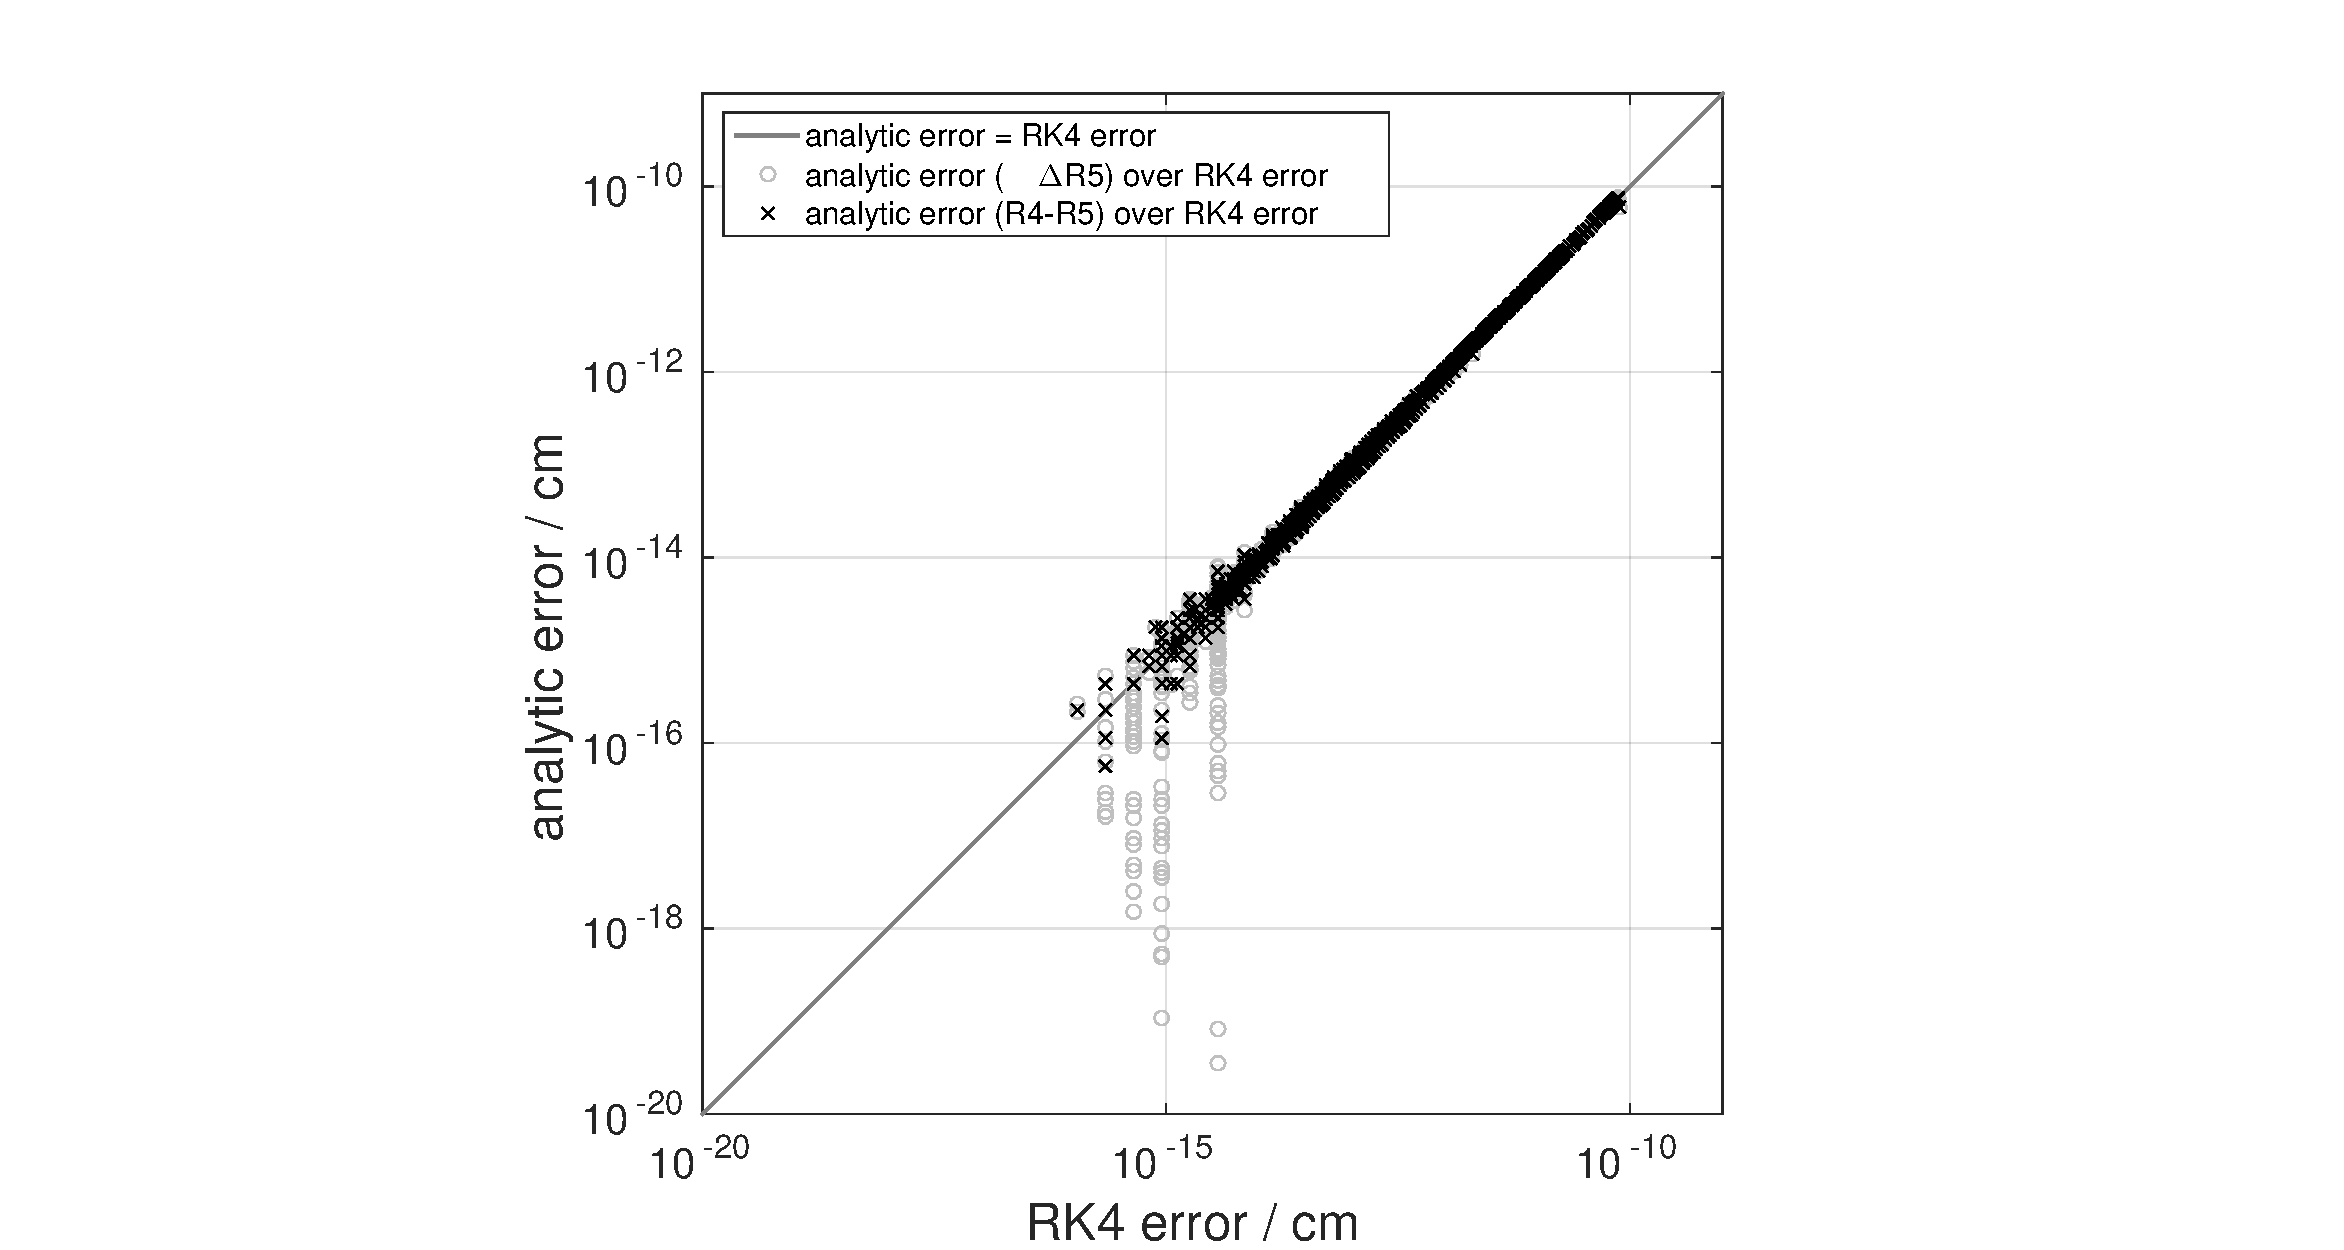
\includegraphics[width=1.2\textwidth]{figures/RK4_alpha555_cyl.pdf}
		\caption{Double-logarithmic plot of two versions for the \textit{analytic error} (difference of fourth and fifth order solution (x), direct computation of fifth order contribution (o)) are hereby plotted as function of the \textit{measured error} for a grid size of $(N_R,N_\varphi,N_Z) = (5,5,5)$, calculations were performed using cylindrical coordinates}  
	\label{fig:RK4_alpha555_cyl}

\vspace{-0.5cm}
%\end{subfigure}
 \hfill%
%\begin{subfigure}[b]{0.48\textwidth}
\end{figure}
\begin{figure}[H]
\centering
%\begin{subfigure}[b]{0.48\textwidth}
\vspace{-0.5cm}
	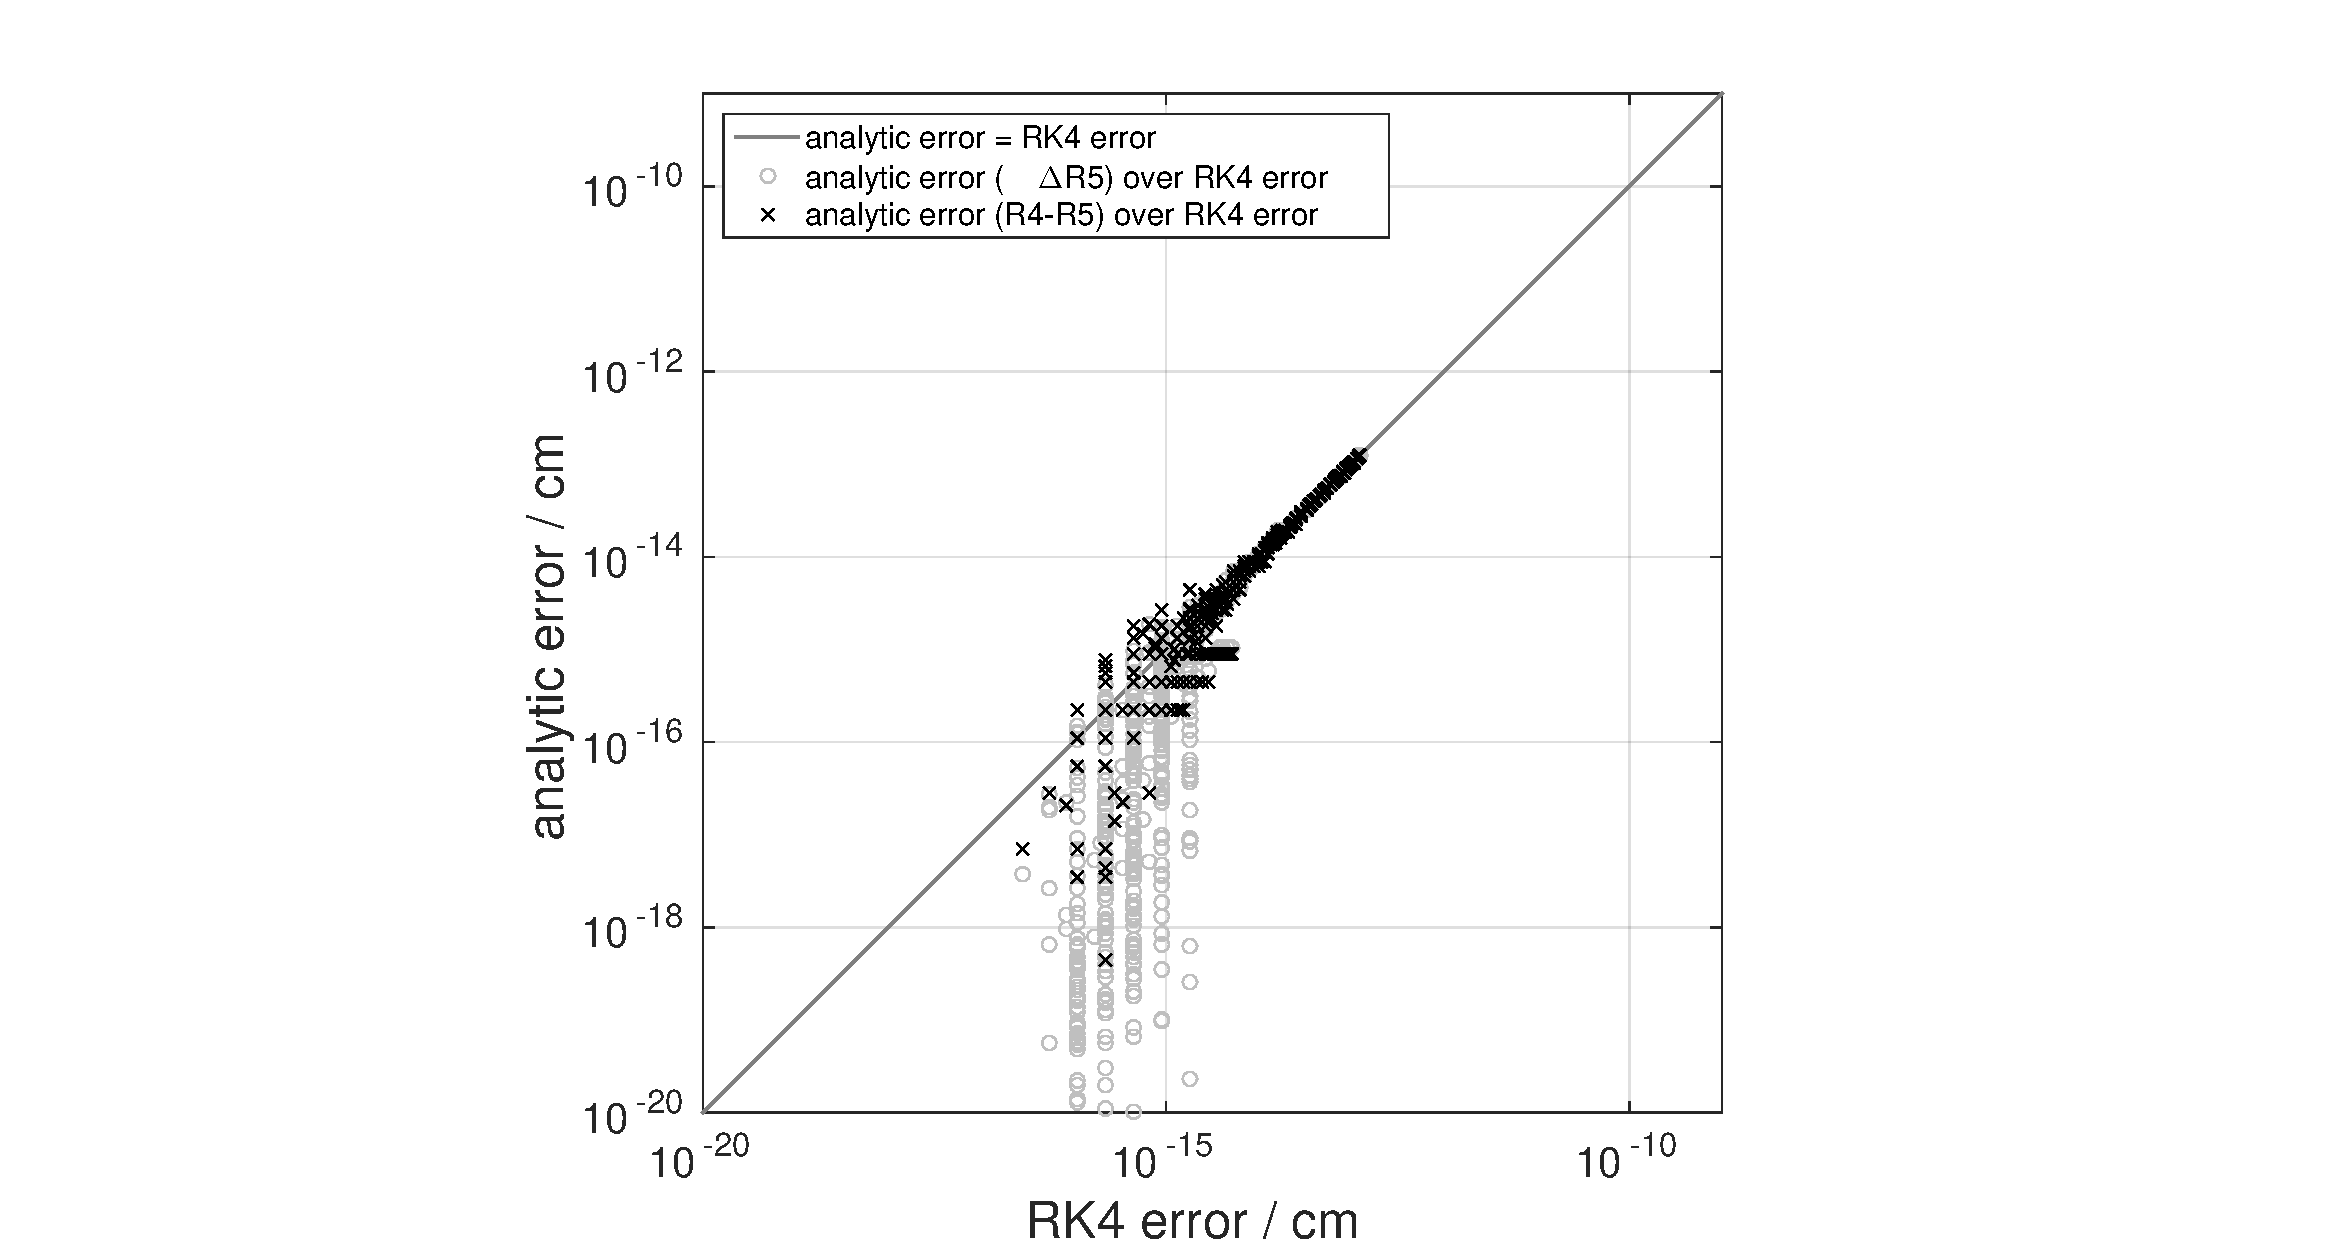
\includegraphics[width=1.2\textwidth]{figures/RK4_alpha121212_cyl.pdf}
		\caption{Double-logarithmic plot of two versions for the \textit{analytic error} (difference of fourth and fifth order solution (x), direct computation of fifth order contribution (o)) are hereby plotted as function of the \textit{measured error} for a grid size of $(N_R,N_\varphi,N_Z) = (12,12,12)$, calculations were performed using cylindrical coordinates}  
	\label{fig:RK4_alpha121212_cyl}

%\end{subfigure}

	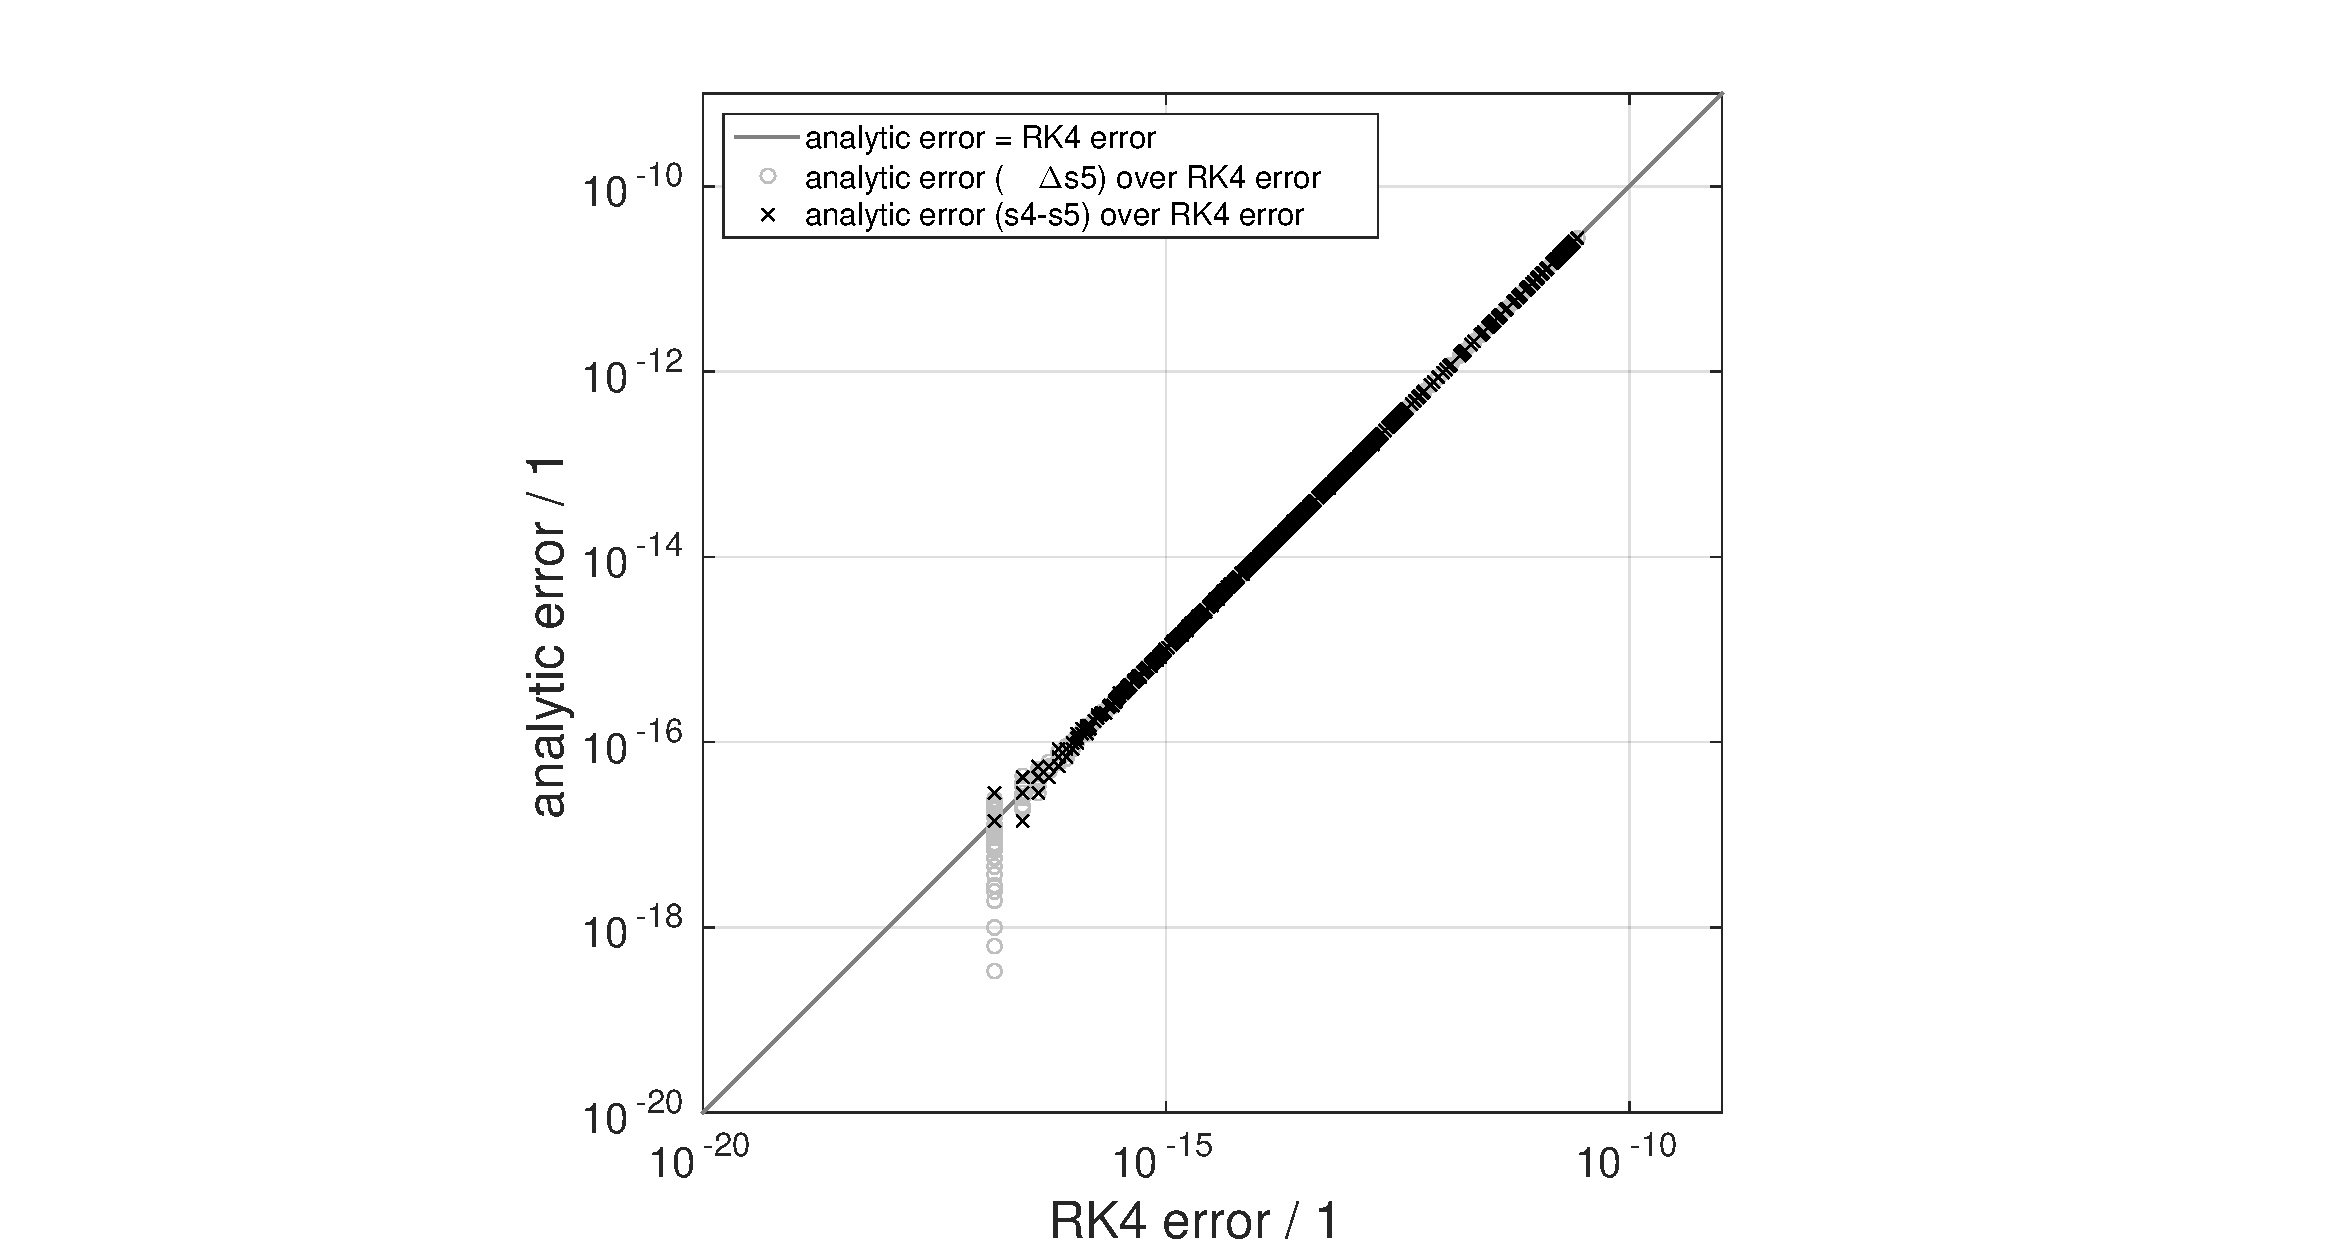
\includegraphics[width=1.2\textwidth]{figures/RK4_alpha555_SFC.pdf}
		\caption{Double-logarithmic plot of two versions for the \textit{analytic error} (difference of fourth and fifth order solution (x), direct computation of fifth order contribution (o)) are hereby plotted as function of the \textit{measured error} for a grid size of $(N_s,N_\vartheta,N_\varphi) = (5,5,5)$, calculations were performed using symmetry flux coordinates}  
	\label{fig:RK4_alpha555_SFC}
\vspace{-0.5cm}
%\end{subfigure}
 \hfill%
 \end{figure}
\begin{figure}[H]
\centering
%\begin{subfigure}[b]{0.48\textwidth}
\vspace{-0.5cm}
%\begin{subfigure}[b]{0.48\textwidth}
	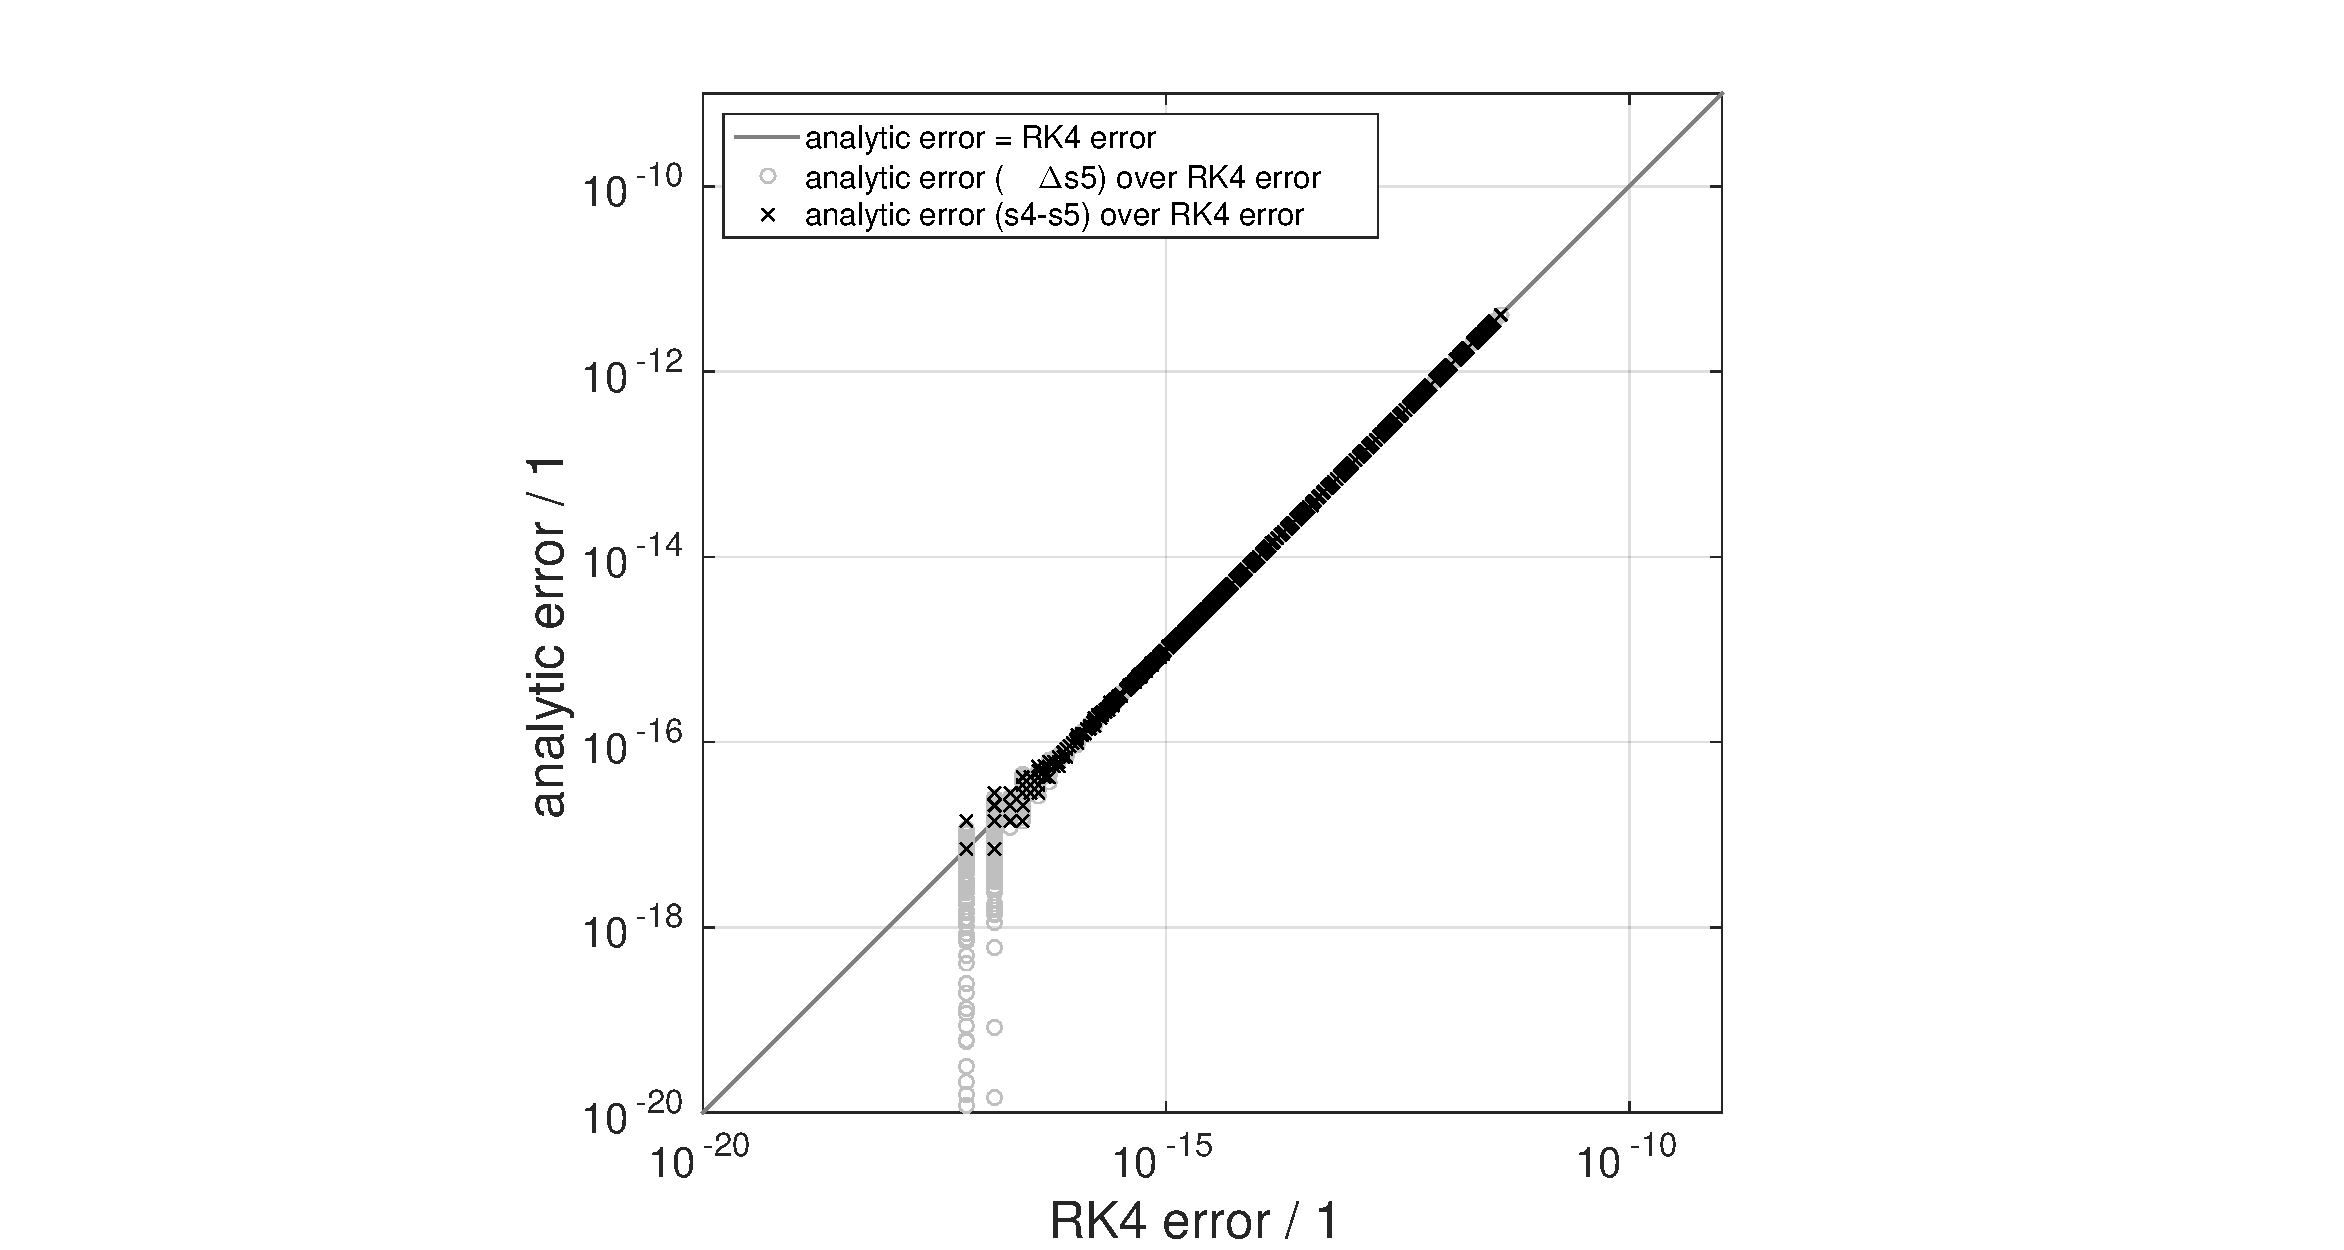
\includegraphics[width=1.2\textwidth]{figures/RK4_alpha121212_SFC.pdf}
		\caption{Double-logarithmic plot of two versions for the \textit{analytic error} (difference of fourth and fifth order solution (x), direct computation of fifth order contribution (o)) are hereby plotted as function of the \textit{measured error} for a grid size of $(N_s,N_\vartheta,N_\varphi) = (12,12,12)$, calculations were performed using symmetry flux coordinates}  
	\label{fig:RK4_alpha121212_SFC}

%\end{subfigure}
\end{figure}


\newpage





%\section{Analytical estimation of RK4 error}
%\label{sec:Analytic_estimation_RK4}
%In section \ref{sec:analytical_solution} the analytic solution to the equations of motion has been derived, it is now of interest to give an analytic estimation for the behavior of the leading order of the derived solution. The result of interest is hereby not expected to accurately represent the error, but rather give a measure for the trend and depence on a few parameters, thus, only the fifth order term of the Taylor expansion for the first component of the axisymmetric solution given in equation \eqref{AxisymmetricAnalyticalExpressionX} will be analyzed in cylindrical coordinates.\\
%\newline
%After calculating the fifth order of the Taylor expansion for eq.~\eqref{AxisymmetricAnalyticalExpressionX}, one is now interested in rewriting these terms in a smart way to make it less tedious to find an analytical estimation. A possible way to write the expression for the fifth order term is 
%
%\be{eq:5th_order_axisymm_R}
%\begin{split}
%\Delta R^{(5)} = &\frac{\lambda^3\tau^5}{120} \left(\lambda \beta_1 \left( 16 v_{\parallel,0}^2 - 30 \frac{b}{\lambda}v_{\parallel,0} + 14 \frac{b^2}{\lambda^2}\right) + \lambda \alpha_1 \left(v_{\parallel,0}-\frac{b}{\lambda}\right)  \right. \\
%&\left. + \frac{cm}{e} u_3 \vec{d_v}\left(-\frac{b}{a}\vec{\alpha}-\vec{\gamma}-\lambda\vec{s_0}\right)  \right)~,\\
%\end{split}
%\ee
%for this derivation, these relations were furthermore used
%\bea*
%\nonumber
%\lambda = \frac{cm}{e} \left( \frac{\partial h_2}{\partial x^3} \frac{\partial U}{\partial x^1} - \frac{\partial h_2}{\partial x^1} \frac{\partial U}{\partial x^3}  \right)~,\\
%\nonumber
%\frac{cm}{e} \frac{\partial h_k}{\partial x^l} = \frac{\partial }{\partial x^l} \left( \frac{B_k}{\omega_c}\right)~,\\
%\nonumber
%\frac{\partial U}{\partial x^i} = - \frac{v_{\perp,e.p.}^2}{2 B_{e.p.}}\frac{\partial B}{\partial x^i}-\frac{e}{m} \frac{\partial \Phi}{\partial x^i}~,\\
%\nonumber
%\beta^1 = -\frac{cm}{e} d_{23}~,\\
%\nonumber
%b = \varepsilon^{ijk} \frac{\partial U}{\partial x^i}\frac{\partial A_k}{\partial x^j} = \left( \frac{\partial U}{\partial x^i}\right)\cdot\underbrace{\left(\frac{\partial A_k}{\partial x^j}\right) }_{\alpha^i}  = \vec{u}_v\cdot \vec{\alpha} ~,\\
%\nonumber
%\gamma^i = \varepsilon^{ijk} \left(\frac{B_k}{\omega_c}\right)_0\frac{\partial U}{\partial x^j}~,\\
%\nonumber
%\vec{d}_v = \begin{pmatrix}
%\frac{\partial h_2}{\partial x^1}\\
%\nonumber
%\frac{\partial h_2}{\partial x^3}
%\end{pmatrix}~,~
%\vec{u}_v = \begin{pmatrix}
%\frac{\partial U}{\partial x^1}\\
%\frac{\partial U}{\partial x^3}
%\end{pmatrix}~,~
%\vec{s}_0 = \begin{pmatrix}
%R_0\\Z_0
%\end{pmatrix}~.\\
%\nonumber
%\eea
%
%By comparing the different terms in equation \eqref{eq:5th_order_axisymm_R}, one can identify
%
%\be{eq:RK4_highest_contributor}
%\frac{\lambda^3 \tau^5}{120}\lambda\beta_1\left(14\frac{b^2}{\lambda^2}\right)
%\ee
%
%as the most significant contributor to the error.
%According to analytical estimations done by Kasilov \ref, the appearing quantities can be approximated by 
%
%\bea{}
%\nonumber
%\beta_1 \approx \frac{cm}{e} \frac{a}{q^2R}~,\\
%\nonumber
%b \approx B v^2\frac{r}{qR}~,\\
%\lambda \approx \frac{v^2B}{\omega_c a} = \rho_L \frac{Bv}{a}~,\\
%\nonumber
%\frac{b}{\lambda} \approx  \frac{v a^2}{qR\rho_L}~.\\
%\nonumber
%\eea
%
%
%
%Using these approximations, \eq{eq:RK4_highest_contributor} can be estimated to
%\be{}
%\Delta R(\tau) = \frac{7}{60} \frac{cm}{e} \frac{\rho^2 B^4 v^6 a}{q^4 R^3} \tau^5 ~.
%\ee
%
%Since $\tau$ roughly scales with the number of grid points in $\varphi$ direction according to
%
%\be{}
%\tau \approx \frac{2\pi}{Bv}\frac{1}{N_\varphi}~,
%\ee
%
%also the Runge Kutta accuracy is expected to be much higher for a finer tetrahedral grid as the average step sizes in $\tau$ decrease proportionately to $1/N_\varphi$ and $\tau$ furthermore being taken to the fifth power.   
%


\end{document}